%  LaTeX support: latex@mdpi.com 
%  In case you need support, please attach all files that are necessary for compiling as well as the log file, and specify the details of your LaTeX setup (which operating system and LaTeX version / tools you are using).

% You need to save the "mdpi.cls" and "mdpi.bst" files into the same folder as this template file.

%=================================================================
\documentclass[entropy,article,submit,moreauthors,pdftex,10pt,a4paper]{mdpi} 
\usepackage{subfigure}

%
%--------------------
% Class Options:
%--------------------
% journal
%----------
% Choose between the following MDPI journals:
% actuators, admsci, aerospace, agriculture, agronomy, algorithms, animals, antibiotics, antibodies, antioxidants, applsci, arts, atmosphere, atoms, axioms, batteries, behavsci, beverages, bioengineering, biology, biomedicines, biomimetics, biomolecules, biosensors, brainsci, buildings, carbon, cancers, catalysts, cells, challenges, chemosensors, children, chromatography, climate, coatings, computation, computers, condensedmatter, cosmetics, cryptography, crystals, data, dentistry, designs, diagnostics, diseases, diversity, econometrics, economies, education, electronics, energies, entropy, environments, epigenomes, fermentation, fibers, fishes, fluids, foods, forests, futureinternet, galaxies, games, gels, genealogy, genes, geosciences, geriatrics, healthcare, horticulturae, humanities, hydrology, informatics, information, infrastructures, inorganics, insects, instruments, ijerph, ijfs, ijms, ijgi, ijtpp, inventions, jcdd, jcm, jdb, jfb, jfmk, jimaging, jof, jintelligence, jlpea, jmse, jpm, jrfm, jsan, land, languages, laws, life, literature, lubricants, machines, magnetochemistry, marinedrugs, materials, mathematics, mca, mti, medsci, medicines, membranes, metabolites, metals, microarrays, micromachines, microorganisms, minerals, molbank, molecules, mps, nanomaterials, ncrna, neonatalscreening, nutrients, particles, pathogens, pharmaceuticals, pharmaceutics, pharmacy, philosophies, photonics, plants, polymers, processes, proteomes, publications, recycling, religions, remotesensing, resources, risks, robotics, safety, sensors, separations, sexes, sinusitis, socsci, societies, soils, sports, standards, sustainability, symmetry, systems, technologies, toxics, toxins, tropicalmed, universe, urbansci, vaccines, vetsci, viruses, water
%---------
% article
%---------
% The default type of manuscript is article, but can be replaced by: 
% addendum, article, book, bookreview, briefreport, casereport, changes, comment, commentary, communication, conceptpaper, correction, conferenceproceedings, conferencereport, expressionofconcern, meetingreport, creative, datadescriptor, discussion, editorial, essay, erratum, hypothesis, interestingimage, letter, newbookreceived, opinion, obituary, projectreport, reply, retraction, review, preprints, shortnote, supfile, technicalnote
% supfile = supplementary materials
%----------
% submit
%----------
% The class option "submit" will be changed to "accept" by the Editorial Office when the paper is accepted. This will only make changes to the frontpage (e.g. the logo of the journal will get visible), the headings, and the copyright information. Also, line numbering will be removed. Journal info and pagination for accepted papers will also be assigned by the Editorial Office.
%------------------
% moreauthors
%------------------
% If there is only one author the class option oneauthor should be used. Otherwise use the class option moreauthors.
%---------
% pdftex
%---------
% The option pdftex is for use with pdfLaTeX. If eps figure are used, remove the option pdftex and use LaTeX and dvi2pdf.

%=================================================================
\firstpage{1} 
\makeatletter 
\setcounter{page}{\@firstpage} 
\makeatother 
\articlenumber{x}
\doinum{10.3390/------}
\pubvolume{xx}
\pubyear{2016}
\copyrightyear{2016}
\externaleditor{Academic Editor: name}
\history{Received: date; Accepted: date; Published: date}

%------------------------------------------------------------------
% The following line should be uncommented if the LaTeX file is uploaded to arXiv.org
%\pdfoutput=1

%=================================================================
% Add packages and commands here. The following packages are loaded in our class file: fontenc, calc, indentfirst, fancyhdr, graphicx, lastpage, ifthen, lineno, float, amsmath, setspace, enumitem, mathpazo, booktabs, titlesec, etoolbox, amsthm, hyphenat, natbib, hyperref, footmisc, geometry, caption, url, mdframed

%=================================================================
%% Please use the following mathematics environments: Theorem, Lemma, Corollary, Proposition, Characterization, Property, Problem, Example, ExamplesandDefinitions, Remark, Definition
%% For proofs, please use the proof environment (the amsthm package is loaded by the MDPI class).

%=================================================================
% Full title of the paper (Capitalized)
\Title{Oriented Gradient Histogram applied to P300 Detection}

% Authors, for the paper (add full first names)
\Author{Rodrigo Ramele $^{1,\dagger}$*, Ana Julia Villar $^{1}$ and Juan Miguel Santos  $^{1}$}
% Authors, for metadata in PDF
\AuthorNames{Rodrigo Ramele, Ana Julia Villar and Juan Miguel Santos}

% Affiliations / Addresses (Add [1] after \address if there is only one affiliation.)
\address[1]{%
$^{1}$ \quad Computer Engineering Department, Instituto Tecnológico de Buenos Aires (ITBA); info@itba.edu.ar}

% Contact information of the corresponding author
\corres{Correspondence: rramele@itba.edu.ar; Tel.: +54-11-2150-4800(5834)}

% Current address and/or shared authorship
\firstnote{Current address: C1437FBH Lavarden 315, Ciudad Autónoma de Buenos Aires, Argentina} 

% Simple summary
%\simplesumm{}

% Abstract (Do not use inserted blank lines, i.e. \\) 
\abstract{The analysis of Electroencephalographic (EEG) signals is of ulterior importance to elucidate patterns that could improve the implementation of Brain Computer Interfaces (BCI). These systems are meant to provide alternative pathways to transmit volitional information which could potentially enhance the quality of life of patients affected by neurodegenerative disorders or improve Human Computer Interaction systems.  Of particular interests are those which are based on the recognition of Event-Related Potentials (ERP) because they can be elicited by external stimuli and used to implement spellers, to control external devices or even avatars in virtual reality environments.  This work mimics what electroencephalographers have been doing clinically, visually inspecting and categorizing phenomena within the EEG by the extraction of features from the images of the plots of the signals.  It also aims to provide a framework to analyze, characterize and classify EEG signals, with a focus on the P300, an ERP elicited by the oddball paradigm of rare events.  The validity of the method is shown by offline processing a public dataset of Amyotrophic Lateral Sclerosis (ALS) patients.}

% Keywords
\keyword{electroencephalography (EEG); BCI; P300; ALS; NBNN; HOG; SIFT}

% The fields PACS, MSC, and JEL may be left empty or commented out if not applicable
%\PACS{J0101}
%\MSC{}
%\JEL{}
%\AMS{}

% If this is an expanded version of a conference paper, please cite it here: enter the full citation of your conference paper, and add $^\S$ in the end of the title of this article.
%\conference{}

%%%%%%%%%%%%%%%%%%%%%%%%%%%%%%%%%%%%%%%%%%
% Only for the journal Data:

%\dataset{DOI number or link to the deposited data set in cases where the data set is published or set to be published separately. If the data set is submitted and will be published as a supplement to this paper in the journal Data, this field will be filled by the editors of the journal. In this case, please make sure to submit the data set as a supplement when entering your manuscript into our manuscript editorial system.}

%\datasetlicense{license under which the data set is made available (CC0, CC-BY, CC-BY-SA, CC-BY-NC, etc.)}

%%%%%%%%%%%%%%%%%%%%%%%%%%%%%%%%%%%%%%%%%%
% For Conference Proceedings Papers: add the conference title here
%\conferencetitle{}

%\setcounter{secnumdepth}{4}
%%%%%%%%%%%%%%%%%%%%%%%%%%%%%%%%%%%%%%%%%%
\begin{document}

%%%%%%%%%%%%%%%%%%%%%%%%%%%%%%%%%%%%%%%%%%
%% Only for the journal Gels: Please place the Experimental Section after the Conclusions

%%%%%%%%%%%%%%%%%%%%%%%%%%%%%%%%%%%%%%%%%%
\setcounter{section}{-1} %% Remove this when starting to work on the template.

\section{Introduction}

%\begin{enumerate}[leftmargin=*,labelsep=3mm]
%\item	Why
%\item	Purpose and significance
%\item	Current state of the research field and key publications cited
%\item   Controversial hypothesis
%\item   Main aim and principal conclusions.
%\end{enumerate}
%
%\begin{enumerate}[leftmargin=*,labelsep=3mm]
%\item El paper tiene un foco general en EEG y rapidamente se centra en BCI como una prueba del método.
%\item La relevancia de estudiar métodos de análisis de EEG para pacientes con ALS.
%\item Ofrece una Receta de cómo implementar un esquema simple de detección de P300 y ofrece una comparativa contra el paper de las italianas.
%\item La transversalidad del método de poder detectar eventos rítmicos asi como transientes como p300.
%\item La posibilidad de utilizarlo para reconocer, fuertemente un patron particular y con la flexibilidad de detectar variantes basado en las poblaciones de descriptores (esta es mi hipótesis de porque funciona, porque yo vi que el método se hace pelota con pequeñas variantes de la señal).
%\item La importancia del averaging de EEG y sus desbalanceos, puntualizando que en el paper original
%\item Que la caída en la clasificación no cae significativamente aún bajando la cantidad de repeticiones requeridas para el averaging.
%\item ¿ Por qué da mejor en PO8 que en Cz y Pz que son los canales P300 ?  (como future work).
%\end{enumerate}


Although recent advances in neuroimagining techniques (particularly radio-nuclear and radiological scanning methods) \citep{Schomer2010} have diminished the prospects of the traditional Electroencephalography (EEG), the advent and development of digitalized devices has pressed for a revamping of this hundred years old technology.  Their versatility, ease of use, temporal resolution, ease of development and fabrication, and its proliferation as consumer devices, are pushing EEG to become the de-facto non invasive portable or ambulatory method to access and harness brain information \cite{DeVos2014}

A key contribution to this expansion has been the field of Brain Computer Interfaces (BCI) \citep{WolpawJonathanR2012} which is the pursuit of the development of a new channel of communication particularly aimed to persons affected by neurodegenerative diseases.

One noteworthy aspect of this novel communication channel is the ability to volitionally transmit information from the Central Nervous System (CNS) to a computer device and from there use that information to control a wheelchair \citep{Carlson2013}, as input to a speller application \citep{Guger2009a}, in a Virtual Reality environment \citep{Lotte2013} or as aiding tool in a rehabilitation procedure \citep{Jure2016}.  The holly grail of BCI is to implement a new complete and alternative pathway to restore lost locomotion \citep{WolpawJonathanR2012}.

EEG signals are remarkably complex and have been characterized as a multichannel non-stationary stochastic process.  Additionally, they have high variability between different subjects and even between different moments for the same subject, requiring adaptive and co-adaptive calibration and learning procedures \citep{Clerc}.  Hence, this imposes an outstanding challenge that is necessary to overcome in order to extract information from raw EEG signals.

Moreover, EEG markers \citep{Clerc} that can be used to volitionally transmit information are limited, and each one of them has a particular combination of appropriate methods to decode them. Inevitably, it is necessary to implement  distinct and specialized algorithmic methods, to filter the signal, enhance its Signal to Noise Ratio (SNR), and try to determine some meaning out of it.  

%Patients suffering from ALS their brain signals do suffer slow and deteriorating changes that may lead to different EEG patterns alterations \citep{Nijboer2009,Riener2014}.


%Besides novel applications of BCI, the goal of the entire discipline is to provide communication assistance to people affected by neuro-degenerative diseases.  It is understood that for people suffering from ALS, even though this pathology do not harm the CNS, their brain signals do suffer slow and deteriorating changes that may lead to different EEG patterns alterations \citep{Nijboer2009,Riener2014}.

BCI has gained mainstream public awareness with worldwide challenge competitions like Cybathlon  \citep{Riener2014} and even been broadcasted during the inauguration ceremony of the 2014 Soccer World Cup.  New developments have overcome the out-of-the-lab high-bar and they are starting to be used in real world environments \citep{Huggins2016}.  However, they still lack the necessary robustness, and its performance is well behind any other method of human computer interaction, including any kind of detection of residual muscular movement~\citep{Clerc}.


In~\citep{Ramele2016},  authors introduce a method for classification of rhythmic patterns using gradient histograms orientations. Inspired in that work, we proposed a novel application of the developed method to classify and describe transient events like those produced by P300 Event Related Potential. 
 Its validity is verified by processing offline data for ALS patients.  
The proposed approach is based on the morphological analysis of the shape of the EEG signal~\citep{Alvarado-Gonzalez2016,Yamaguchi2009} and it was built by mimicking what traditionally electroencephalographers have been performing for almost a century: visually inspecting  raw signal plots~\citep{Hartman2005}.

This paper reports a method to, (1) classify P300 signals based on the identification of their structure in the shape domain using histograms of oriented gradients extracted from the image of signal plots, and (2) describe the way in which this classification can be used to implement an offline P300-based BCI Speller application using two public datasets.

This article unfolds as follows: in Section \ref{Feature} the Feature Extraction based on Histogram of Gradients of the Signal Plot method is explained. Section \ref{Preprocessing} and \ref{Pipeline} describe the processing pipeline.  Section \ref{Plot}  clarifies how the image of the signal plot is constructed whereas Section \ref{SIFT}  describes in detail the feature extraction procedure.  Section \ref{Classification}  presents the classification algorithm based on Naive Bayes Near Neighbor  and the final Section shows results and discussion where we expose our remarks, conclusions and future work.

%\subsection{Morphological Signal Analysis}
%
%Several approaches and methods have been applied to decode them.  Of particular interests are morphological signal analysis 
%CITE (Paper del chabon del ITBA que detalla bien los diferentes metodos) \citep{Alvarado-Gonzalez2016,Yamaguchi2009}.
%
%Morphological or 
%
%template matching
%
%spike
%sharp wave
%spike wave
%polyspike 
%slow wave complex
%
%shape domain
%
%\subsection{P300}
%
%Uhhhh I can talk a lot about P300 \citep{Knuth2006}.
%
%P300 single trial is a golden grail of Brain computer interfaces.  It is studied and analyzed in this way, here in this other way, in this other way is here.

\section{Materials and Methods}

\subsection{Feature Extraction based on Histogram of Gradients of the Signal Plot} \label{Feature}

The P300~\citep{Farwell1988,Knuth2006} is a positive deflection of the EEG signal which occurs around $300$ ms after the onset of a rare and deviant stimulus that the subject is expected to attend.  It is produced under the oddball paradigm~\cite{WolpawJonathanR2012} and it is consistent across different subjects. It has a lower amplitude  ($\pm 5 \mu V $) compared to basal EEG activity, reaching a SNR of around $-15$ db estimated based on the amplitude of the P300 response signal divided by the standard deviation of the background EEG activity~\citep{Hu2010}.  This signal can be used to implement a speller application by means of a Speller Matrix~\citep{Farwell1988}. Fig.~\ref{fig:p300matrix} shows an example of a Speller Matrix used in the OpenVibe Open Source software~\citep{Renard2010}, where the flashings of rows and columns provide the deviant stimulus required to elicit this physiological response.   Each time a row or column that contains the desired letter flashes, the corresponding synchronized EEG signal should also contain the P300 signature and by detecting it, the selected letter can be identified.

\begin{figure}[H]
\centering
\subfigure[Row flash.]{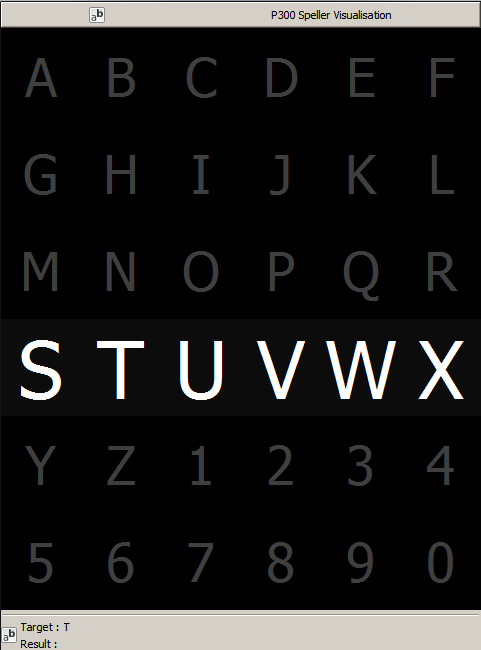
\includegraphics[width=.29\linewidth]{openvibep300matrix.png}}
\subfigure[Column flash.]{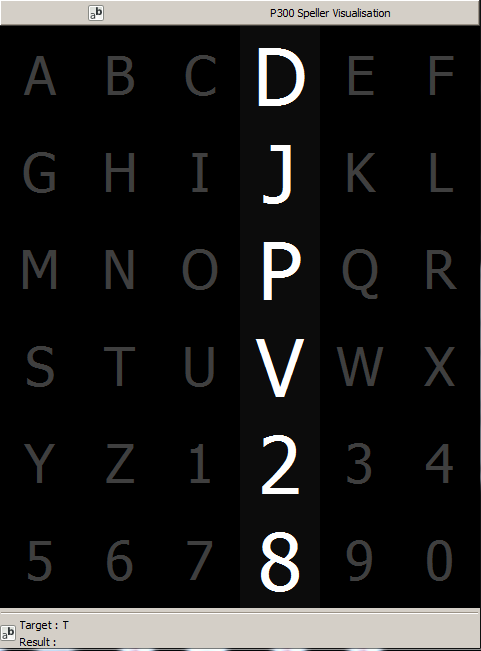
\includegraphics[width=.29\linewidth]{p300matrixcoloriginal.png}}
\caption{Example of a Speller Matrix.  Rows and columns flash intermittently in random permutations.}
\label{fig:p300matrix}
\end{figure}

%The proposed algorithm was designed to perform specifically this decoding.

% of the selected letter based on the detection of the P300 Event Related Potential response on the corresponding EEG signal.  

\subsubsection{Preprocessing} \label{Preprocessing}

The first step consists of the enhancement of the SNR of the P300 pattern above the level of basal EEG. 
The processing pipeline starts by applying a notch filter to the raw signal, a 
$4$th degree $10$ Hz lowpass Butterworth filter and finally a decimation with a Finite Impulse Response (FIR) filter of order $30$ from the original sampling frequency down to $16$ Hz \citep{Krusienski2006}.

\subsubsection{Processing Pipeline} \label{Pipeline}

\begin{itemize}
\item \textbf{Artefact Removal}: The EEG signal matrix is processed on a channel by channel basis.   For every 12 flashing stimuli, i.e. one complete sequence of intensification of each of the $6$ rows plus the $6$ columns, a basic artefact elimination procedure is implemented by removing the entire sequence when any signal deviates above/bellow $ \pm 70 \mu V $.
\item \textbf{Segmentation}: For each of the $12$ stimuli,  a window of $1$ second of the multichannel signal is extracted, starting from the stimulus onset, corresponding to each row/column intensification.  Two of these segments are labeled as \textit{hit}, whereas the remaining $10$ are labeled as \textit{no hit}.  A hit represents that the EEG segment should contain the P300 ERP signature time-locked to the flashing stimulus. 
\item \textbf{Signal Averaging}:  The P300 ERP is deeply buried under background EEG so the traditional approach to identify it is by point-to-point averaging the time-locked stacked signal segments.  Hence the values which are not related to, and not time-locked to the onset of the stimulus are canceled out \citep{Liang2008}. 
\end{itemize}

This last step determines the operation of any P300 Speller.  In order to obtain an improved signal in terms of its SNR, repetitions of the sequence of row/column intensification are necessary.  And, at the same time, as long as more repetitions are needed, the ability to transfer information faster is diminished, so there is a trade-off that must be acutely determined.

\subsubsection{Signal Plotting} \label{Plot}

The underlying idea of this method is to generate a template for the signal \citep{Ramele2016},  based on the image plot.  Hence, the first step is the signal transformation into a temporary binary image.

Averaged signal segments obtained from the preprocessing stage are first scaled and standardized (i.e. z-score) by 

\begin{equation}
\tilde{x}(t,c) = \left \lfloor{ \gamma \cdot \frac{( x(t,c) - \bar{x}(c)  )}{ \sigma(c) } }\right \rfloor
\end{equation}

\noindent where $\gamma$ is the image scale, $t$ is time and $ x(t,c) $ is the point-to-point averaged EEG matrix for time $t$ and for  channel $c$. Lastly, $\bar{x}(c)$ and $ \sigma (c) $ are the mean and standard deviation of $x$.

Consequently, the image is constructed by placing the sample points according to

\begin{equation}
I(z_1,z_2) = \left\{ \begin{array}{rl}
255 & \text{if} \,  z_1 = \gamma \cdot t; z_2 = \tilde{x}(t,c) + z(c) \\
0   & \mbox{otherwise}
\end{array}\right.
\label{eq:images}
\end{equation}

\noindent where $ z_1$ and $z_2$ iterate over the width (based on the length of the signal segment) and height (based on the peak-to-peak amplitude) of the newly created image.  The function $z(c)$ is the \textit{zerolevel} which is the location on the image where the signal's zero value should be located in order to fit the entire signal within the image:

\begin{equation}
z(c) = \left \lfloor{ \frac{\max \tilde{x}(t,c)  - \min \tilde{x}(t,c) }{2} }\right \rfloor -   \left \lfloor{ \frac{\max \tilde{x}(t,c)  + \min \tilde{x}(t,c)}{ 2} }\right \rfloor
\label{eq:zerolevel}
\end{equation}
  

In order to complete the plot from the pixels, the Bresenham \citep{Bresenham1965,Ramele2016} algorithm is used to interpolate straight lines between each pair of  consecutive pixels.

%\noindent and is used to derive local representations that captures the visual shape of the signal.

\subsubsection{Feature Extraction: Histogram of Oriented Gradients}
\label{SIFT}

%is calculated on local image patches centered on sample points \citep{Vedaldi2010}.

On the generated image, a keypoint $\mathbf{kp}$ is placed on a pixel $(x_{kp}, y_{kp})$ over the image plot and a window around the keypoint is considered. A local image patch is constructed by dividing the window in $16$ blocks of size $3s$ each one,  where $s$ is the scale of the local patch and it is an input parameter of the algorithm. It is arranged in a $4 \times 4$ grid and the pixel $ \mathbf{kp}$ is the patch center. 

A local representation of the shape of the signal within the patch can be described by obtaining the gradient orientations on each of the $16$ blocks and creating a histogram of gradients.  This technique is based on Lowe's SIFT~\citep{Lowe2004} method, and it is biomimetically inspired in how the visual cortex detects shapes by analyzing orientations.   In order to calculate the histogram, the interval $[0-360]$ of possible angles is divided in $8$ bins, each one at $45$ degrees.

 For each spacial bin $ i,j = \{1,2,3,4\} $, corresponding to the indexes of each block $B_{i,j}$,  the orientations are accumulated in a  $3$-dimensional histogram $h$ through the following equation: 
 

\begin{equation}
 h(\theta,i,j) = 3s \sum_{\mathbf{x} \in B_{i,j}} w_\mathrm{ang}(\angle J(\mathbf{x}) - \theta)\, w_{ij}\left(\frac{\mathbf{x} - \mathbf{kp}}{3 s}\right)\, |J(\mathbf{x})|
\label{eq:histogram}
\end{equation}

\noindent  where $ \theta \in \{0, 45, 90, 135, 180, 225, 270, 315\} $, $ i,j \in \{1,2,3,4\} $, $ |J(\mathbf{x})| $ is the norm of the gradient vector found at each block of the patch using finite differences, $\angle J(\mathbf{x}) $ is the angle of the gradient vector,  $\theta$ is the angle bin, $\mathbf{x}$ is a pixel from  the $i,j$-block $B_{i,j}$ and $ w_\mathrm{ang}(\cdot) $  and $ w_{ij}(\cdot) $ are linear interpolation functions used by Lowe and Vedaldi et al. in~\citep{Lowe2004,Vedaldi2010}.  Lastly, the fixed value of $ 3 $ is a magnification factor which corresponds to the number of pixels per each block when $s = 1$.  As the patch is of size $4 \times 4$ and  $8$ bin angles are considered, a descriptor of $128$ dimension is obtained. It can be observed that in each step, the histogram is computed by multiplying by $ |J(\mathbf{x})| $ , so the method considers both, the magnitude and the orientation of the gradient vector. 


Fig.~\ref{fig:sampledescriptor} shows an example of a patch and a scheme of the histogram computation. Fig.~\ref{patch} is a plot of the signal and the patch centered in the keypoint. In Fig.~\ref{histogrambines} the possible orientations on each patch are illustrated. They form the corresponding $\mathbf{kp}$-descriptor of $128$ coordinates. The first two blocks are shown.  Following this procedure for every assigned keypoint, we obtain $N_{kp}$ descriptors.
 

 
\begin{figure}[H]
\centering
\subfigure[Plot of the signal, a keypoint and the corresponding patch.]{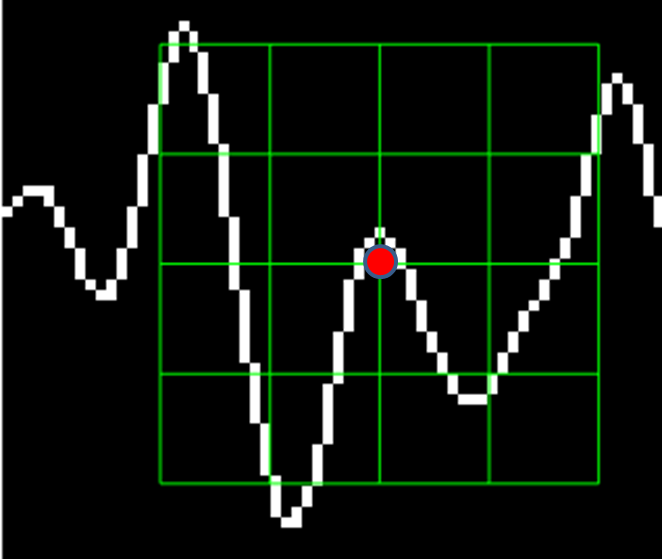
\includegraphics[width=.49\linewidth]{signalpatchkeypoint.png}\label{patch}}
\subfigure[Orientations on two blocks of the patch.]{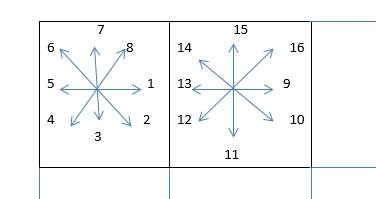
\includegraphics[width=.49\linewidth]{histogramsbines.png}\label{histogrambines}}
%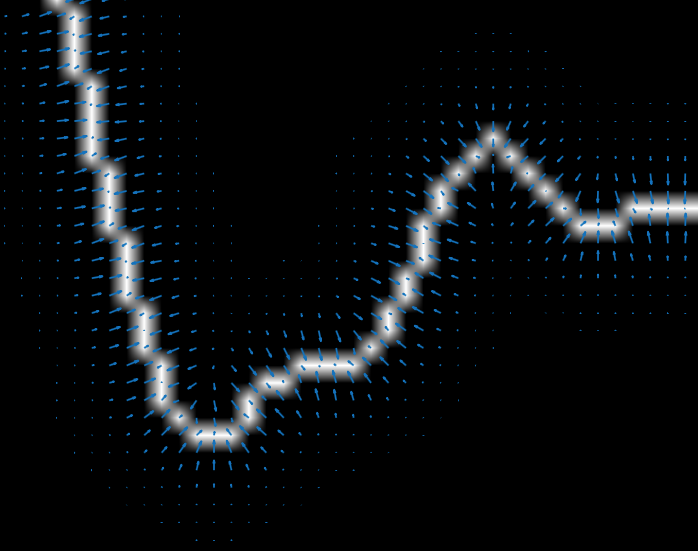
\includegraphics[width=9cm]{gradientszoom.png}
\caption{ Example of a patch and a scheme of the orientation's histogram computation.}
\label{fig:sampledescriptor}
\end{figure}

\subsubsection{Speller Matrix letter Identification}
\label{Classification}

%The following step is classify the descriptors $\{d_{kp}, kp =1,\dots, 12\}$ in order to determine the correct row and column of the chosen letter on the Speller Matrix.   The classification is carried out by using a discriminative semi-supervised classification method, based on the Naive Bayes Nearest Neighbor (NBNN)~\citep{Boiman2008}.

The aim is to identify the selected letter from the matrix. Previously, during training phase, descriptors from labeled segments are extracted.  These descriptors are the P300 templates which are grouped in a template set called $ T $.  Rows are labeled 1-6, whereas columns are labeled 7-12.  The process has the following steps:


\begin{enumerate}
\item Highlight randomly the rows and columns from the matrix.  There is one row and one column that should match the letter selected by the subject.
\item Repeat item 1 $k_a$ times, obtaining the single trial segments $S_1(t,c),\dots,S_{k_a}(t,c)$, where the variables $t$ and $c$ correspond to time and chanel, respectively. The parameter $k_a$ is an input of the algorithm.
\item Compute  
\begin{equation}
x(t,c)= \frac{1}{k_a}\sum_{i=1}^{k_a}S_i(t,c)
\label{averaging}
\end{equation}  

\item Plot the signal $x(t,c)$, according Section~\ref{Plot}.

\item Obtain the descriptor from the image of the signal plot of $x(t,c)$ according to the method described in Section~\ref{SIFT}, $ d^r_1, \dots,  d^r_6 $ for rows and  $ d^c_7, \dots,  d^c_{12} $ for columns. 



\item Match with the Template $T$ by computing  

\begin{equation}
\hat{r} = \arg \min_{u \in \{1,\dots,6\}} \sum_{q \in NN_T(d^r_u)}^{} \left\lVert q -  d^r_u \right\rVert ^2
\label{eq:multiclassificationrow}
\end{equation}

\noindent and

\begin{equation}
\hat{c} = \arg \min_{u \in \{7,\dots,12\}} \sum_{q \in NN_T(d^c_u)}^{} \left\lVert q -  d^c_u \right\rVert ^2
\label{eq:multiclassificationcol}
\end{equation}

where $NN_T(d^l_u), \;l=r,c$ is the set of the $k$ nearest neighbors to $d^l_u, \;l=r,c$ and $q$ is a template descriptor that belongs to $NN_T(d^l_u), \;l=r,c$.  By computing the aforementioned equations, the letter of the matrix can be determined from the intersection of the row $ \hat{r} $ and column $ \hat{c} $. The  $k$ value is an input parameter of the algorithm. 

% By reversing the roles of the query and the class in equations \ref{eq:multiclassificationrow} and \ref{eq:multiclassificationcol}, it is only necessary to obtain the template set $ T $ with the learned descriptors representative of the P300 ERP, hence avoiding the problem of unbalanced classes. 
%The first step consists in extracting labeled \textit{hit} descriptors from the training set which are thus grouped together in a KD-tree \citep{Vedaldi2010} template set $ T $.  On decoding stage, 12 new images from the signal segments are generated, and their descriptors extracted.  The 12 descriptors are divided in rows and columns.  For each one of the 6 query descriptors $ q $ for row/column, its $ k $ nearest neighbours in the template set $T$, $ NN_T^k(q) $ (acquired during the training phase)  are obtained and the distance between each one of them, $ x_i $, and the query descriptor $ q $ is summarized.  The query descriptor $ q $ that minimizes this summation is the one that is chosen, first among the 6 rows, and then among the remaining 6 columns.  By performing this procedure, the correct letter can be identified by matching the row $ r $ and column $ c $ from the P300 speller matrix.   

\end{enumerate}

Figure~\ref{fig:classification} shows a schema of this process. 
\begin{figure}
\centering
\includegraphics[width=15cm]{classificationgraph.pdf}
\caption{Single trial segments are averaged for the 6 rows and 6 columns.}
\label{fig:classification}
\end{figure}

%In the case of the P300 response, the oddball paradigm requires that one of the stimuli be infrequent. Hence this forces the data to be unbalanced~\citep{Tibon2015}.  At the same time, the NBNN method suffers from biased classification on unbalanced classes~\citep{Fornoni2014}. %Para solucionar este problema, 


%Este párrafo no se entiende nada
%------------------

%------------------
\subsection{Experimental Protocol} \label{Protocol}

To verify the validity of the proposed framework and method, the public dataset 008-2014~\citep{Riccio2013} published on the BNCI-Horizon website~\citep{Brunner2014} by  IRCCS Fondazione Santa Lucia, is used. An own dataset with  the same experimental conditions is generated. Both of them are utilized to perform an offline BCI Simulation to decode the spelled words from the provided signals. 

The algorithm was implemented using  VLFeat~\citep{Vedaldi2010} Computer Vision libraries on MATLAB V2014a (Mathworks Inc., Natick, MA, USA). 

In the following sections the characteristics of the datasets and parameters of the identification algorithm are described. 

\subsubsection{P300 ALS Public Dataset}

The experimental protocol used to generate this dataset is explained in~\citep{Riccio2013} but can be summarized as follows:  8 subjects with confirmed diagnoses but on different stages of ALS disease, were recruited and accepted to perform the experiments. The P300 detection task designed for this experiment consisted of spelling 7 words of 5 letters each, using the traditional P300 Speller Matrix~\citep{Farwell1988}. The flashing of rows and columns provide the deviant stimulus required to elicit this physiological response.  The first 3 words are used for training and the remaining 4 words, for testing with visual feedback.  A trial, as defined by the BCI2000 platform~\citep{Schalk2004}, is every attempt to select a letter from the speller. It is composed of signal segments corresponding to $k_a =10$ repetitions of flashes of 6 rows and $k_a =10$ repetitions of flashes of 6 columns of the matrix, yielding 120 repetitions.  Flashing of a row or a column is performed for 0.125 s, following by a resting period (i.e. Inter-stimulus interval) of the same length.  After 120 repetitions an inter-trial pause is included before resuming with the following letter.

The recorded dataset was sampled at 256 Hz and it consisted of an EEG matrix for electrode channels Fz,Cz,Pz,Oz,P3,P4,PO7 and PO8, identified according to the 10-20 International System,  for each one of the 8 subjects.  

%Este párrafo no se entiende nada y repite in order
In order to asses and verify the identification of the P300 response, subjects are instructed to perform a copy-spelling task. They have to fix their attention to successive letters for copying a previously determined set of words, in contrast to a free-running operation of the speller where each user decides on its own what letter to choose.

\subsubsection{Parameters}

Parameters are selected according to the experimental protocol. As the P300 event latency and amplitude vary greatly between subjects, it is necessary to provide a patch that will be able to capture an entire transient event.  Equations~\ref{eq:mapping1} and~\ref{eq:mapping2} can be used to map the original signal parameters to local image patch structure. 
%¿Qué es s? hay que hacer acordar. 
\begin{equation}
s= \frac{\Delta \mu V}{4 \cdot 3} \cdot \gamma 
\label{eq:mapping1}
\end{equation}

\begin{equation}
s = \frac{\lambda \cdot Fs}{4 \cdot 3} \cdot \gamma
\label{eq:mapping2}
\end{equation}
%falta definir gamma
\noindent where $\Delta  \mu V $ corresponds to the amplitude in microvolts that can be covered by the height of the patch, $ Fs $ is the sample frequency of the EEG signal (downsampled to 16 Hz) and $ \lambda $ is the length in seconds covered by the patch. 
% estos son los parámetros que vos usaste en tu experimento? 
By using $ s = 3 $ and a quadruple scale of the image $ \gamma = 4 $ this gives the local patch, and the descriptor, the ability to identify events of 9 $ \mu V $ of amplitude, a resolution of $ 1 $ Pixel $ = \frac{1}{4} \mu V $ and span   of $ \lambda = 0.56 s $ (because the patch is a geometric square, $ s $ must be the same to map both the height and the required span of the signal).  Finally, descriptor locations $\mathbf{kp}$  were selected at $ x =  0.55 s \cdot Fs \cdot \gamma = 35 $ and $ y = z(c) $ (Eq. \ref{eq:zerolevel}). %demasiado larga la frase, no se puede leer.

% esta figura no está comentada en el texto.
\begin{figure}[H]
\centering
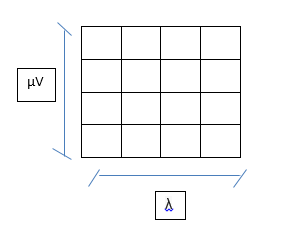
\includegraphics[width=10cm]{localpatch.png}
\caption{The local patch captures the signal information based on both the vertical and horizontal scale.}
\label{fig:sampledescriptor2}
\end{figure}

\subsubsection{P300 for healthy subjects}

We replicat the experiment on healthy subjects using g.Tec g.Nautilus 8 channels.  The experiment protocol is  the same and we 20 subjects, age $ 30$, 5 females and 15 males, 6 right handed and the remaining left handed. 

Participants were recruited voluntarily and the experiment were conducted under anonymous information in accordance with the declaration of Helsinki.  No monetary compensation was delivered and all participants agreed and signed a written informed consent.  All healthy participants had normal or corrected-to normal vision and no history of neuropsychiatric disorders. The experiment was performed with 13 subjects, 7 males, 6 females, average age 22.5 years, standard deviation  1,8 years, range 21–26 years.

EEG data were recorded from the same 8 electrodes positions (C3, Cz, C4, CPz, P3, Pz, P4, POz) with all the systems. The reference positions were placed at the right ear. The ground positions was placed at the left ear, except with the g.Nautilus system (placed at AFz, because this could not be changed). Sampling rate was set at 250 Hz, the closest possible to predefined g.Mobilab sampling rate (256 Hz). Data were acquired notch filtered at 50 Hz and passband filtered between 2 Hz and 30 Hz. The filtering was performed via the proprietary Simulink HighSpeed Online Processing block modules for g.MOBIlab and g.Nautilus systems, and via MATLAB code for the Xpress system. Table~\ref{tab:results} summarizes the acquisition settings for each system.



%8 gel-based active electrodes (g.LADYbird) + g.LADYbird (GND) + g.GAMMAearclip (REF) C3, Cz, C4, CPz, P3, Pz, P4, POz, GND: AFz, REF: right ear


%%%%%%%%%%%%%%%%%%%%%%%%%%%%%%%%%%%%%%%%%%
\section{Results and Discussion} \label{Results}
\label{section:results}
In Figure \ref{fig:subjectaveraged} the grand average (point-to-point) for all the subjects using the information from all the segments can be shown.  The P300 characteristic curve can be seen particularly in subjects 2, and 6 and in a lesser extend in the remaining subjects. In order to correctly decode the selected letter from each trial, particular care was observed to avoid unbalanced number of epochs  (i.e. an unequal number of epochs on each condition), because that may introduce bias in the classification procedure (the variance of averaged signals is inversely proportional to the number of samples and the procedure would be discriminating signals with different variances).  

\begin{figure}[H]
\centering
\includegraphics[width=16cm]{subjectaveraged.eps}
\caption{Point-to-point grand averages of epochs obtained for hits (solid line) and no hits (dashed line) for each one of the 8 subjects for channel Cz. The P300 characteristic curve can be well identified particularly on subjects 2 and 6.}
\label{fig:subjectaveraged}
\end{figure}

Results are shown in Table \ref{tab:results} where the percentage of correctly spelled letters is calculated while performing an offline BCI Simulation.  From the 7 trials for each subject, the first 3 were used as training, and the remaining 4 for testing.  The best performing channel is informed as well.  It is of particular interest that using this method, the best performing channel was not always Cz, and instead occipital channels PO8 and PO7 showed higher performances \citep{Huggins2016,Jure2016}.


\begin{table}[H]
\caption{Percentage of correctly predicted letters while performing an offline BCI Simulation for the best performing channel for each subject. Chance level is 0.02 }
\centering
%% \tablesize{} %% You can specify the fontsize here, e.g.  \tablesize{\footnotesize}. If commented out \small will be used.
\begin{tabular}{ccc}
\toprule
\textbf{Participant}	&  \textbf{BPC}	& \textbf{Performance}\\
\midrule
1     &     Cz   &   0.35  \\
2     &     Fz   &   0.85  \\
3     &     Cz   &   0.25  \\
4     &     PO8 &   0.55  \\
5     &     PO7 &   0.40 \\
6     &     PO7 &   0.60  \\
7     &     PO8 &   0.80  \\
8     &     PO7 &   0.95 \\

\bottomrule
\end{tabular}
\label{tab:results}
\end{table}

The ITR, or BTR, in the case of reactive BCIs \citep{WolpawJonathanR2012} strongly depends on the amount of signal averaging required to transmit a valid and robust selection.  The Performance curves (Fig. \ref{fig:performance}) show how the percentage of correctly identified letters depends on the number of repetitions that were used to obtain the averaged signal.

\begin{figure}[H]
\centering
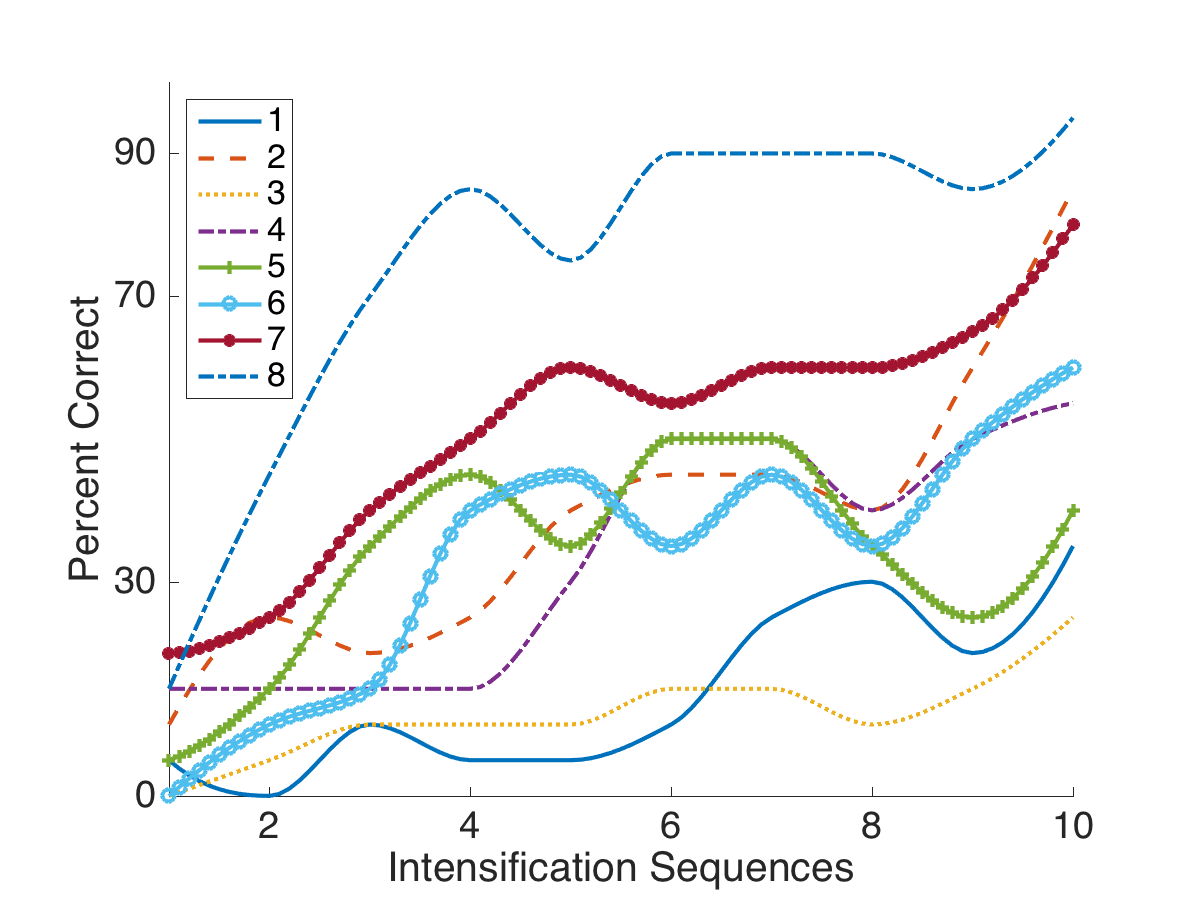
\includegraphics[width=10cm]{performance.eps}
\caption{Performance curves for the eight subjects included in the published dataset.  Three out of eight subjects achieved the necessary performance to implement a valid P300 speller.}
\label{fig:performance}
\end{figure}

We found that only by using the visual aspect of the P300 signal plot,  for some subjects it was not possible to find templates that could allow the classification to reach a higher level.  We hypothesize that as subjects may have different latencies and amplitudes of the P300 signal \citep{Riccio2013}, it may also be the case that the shape of the generated ERP may vary greatly in an intra-subject manner, thus the pattern could not be well generalized and a higher performance could not be reached (Fig.  \ref{fig:p300templates}).

\begin{figure}[H]
\centering
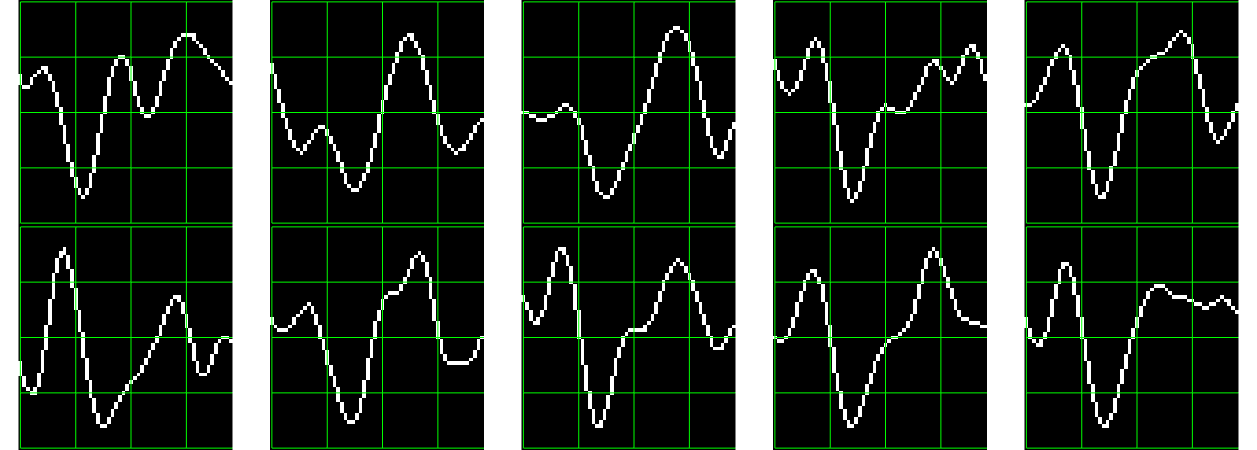
\includegraphics[width=10cm]{subject8.png}
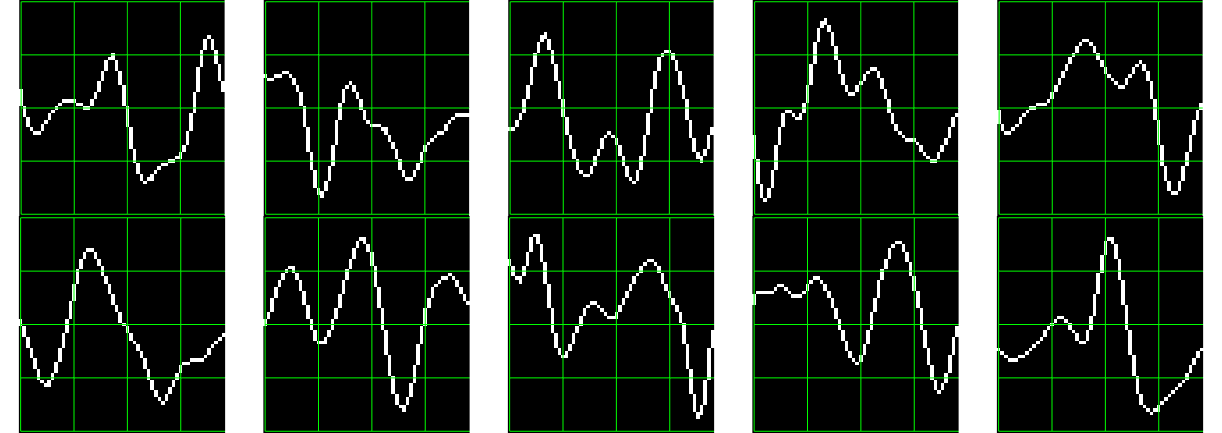
\includegraphics[width=10cm]{subject3.png}
\caption{Ten P300 template patches found for subjects 8 (up) and 3(down).  In coincidence with the performance results, the P300 signature is more clear and consistent for subject 8 (higher performance) while for subject 3 (lower performance) the characteristic pattern is much more difficult to perceive.}
\label{fig:p300templates}
\end{figure}



%%%%%%%%%%%%%%%%%%%%%%%%%%%%%%%%%%%%%%%%%%
%\section{Discussion}
%
%This method, different from other methods which is based on the nonlinearity of the gradient of histograms which can be used to detect 
%
%
%is also based on how the image look like.
%
%SNR of p300 and how to detect it
%
%Check if you can use this to detect any kind of transient signal.
%
%Compare if it is possible with the descriptors from one subject, discriminate the others.
%
%Channal identification based on the metric distance between the bags
%
%Signal Averaging.

%%%%%%%%%%%%%%%%%%%%%%%%%%%%%%%%%%%%%%%%%%
\section{Conclusion}

A method to characterize and classify EEG signals where their characterization is transient in time-space, like the P300 ERP, has been presented.   

%Databases of descriptors.  Flexibility of the descriptor in terms of configuration and size (reference variants of SIFT on lower dimensiones).

The adaptive behaviour of the algorithm make it well suited when the shape of the pattern elicited by the P300 response does not conform to the predicted structure.  This is due to the fact that the descriptors are directly based on how the signals behave in shape domain (i.e. \textit{how actually they looked like}) for the training and calibration step, and they do not require any prior knowledge about the signal.   In contrast, when the shape of the ERP response is not consistent across the same subject, this method would not be able to find the templates and speller performance could be penalized.  

At the same time, by analyzing the generated descriptors, which map in a very detailed and synthetic structure the shape information contained within the patch, a metric about the consistency of the shape of the generated P300 response could also be derived.  It may be worthy of further consideration to evaluate if there is any correlation between the lower performance obtained for some subjects and the characterization of their ALS stage.

We believe that the expanding and the understanding of this tool in order to automatically classify those patterns in EEG that are specifically identified by their shapes (e.g. K-Complex, Vertex Waves, Positive Occipital Sharp Transient \citep{Hartman2005}) is a prospect future work to be considered.  It may also provide  assistance to physician or electroencephalographers to help them locate these EEG patterns particularly in long recording periods, frequent in sleep research.

Moreover, this method can be used as an alternate \textit{BCI predictor} \citep{Clerc}, i.e. to detect BCI illiteracy or to predict the achievable performance of a given method, or even as a tool for artefact removal (which is performed on many occasions by visually inspecting the signal).

%%%%%%%%%%%%%%%%%%%%%%%%%%%%%%%%%%%%%%%%%%
%\subsection{Subsection}
%
%\subsubsection{Subsubsection}
%
%Bulleted lists look like this:
%\begin{itemize}[leftmargin=*,labelsep=4mm]
%\item	First bullet
%\item	Second bullet
%\item	Third bullet
%\end{itemize}
%
%Numbered lists can be added as follows:
%\begin{enumerate}[leftmargin=*,labelsep=3mm]
%\item	First item
%\item	Second item
%\item	Third item
%\end{enumerate}
%
%The text continues here.



%%%%%%%%%%%%%%%%%%%%%%%%%%%%%%%%%%%%%%%%%%
\vspace{6pt} 

%%%%%%%%%%%%%%%%%%%%%%%%%%%%%%%%%%%%%%%%%%
%% optional
%\supplementary{The following are available online at www.mdpi.com/link, Figure S1: title, Table S1: title, Video S1: title.}

%%%%%%%%%%%%%%%%%%%%%%%%%%%%%%%%%%%%%%%%%%
\acknowledgments{This project was supported by the ITBACyT-15 funding program issued by ITBA University.}

%%%%%%%%%%%%%%%%%%%%%%%%%%%%%%%%%%%%%%%%%%

%%%%%%%%%%%%%%%%%%%%%%%%%%%%%%%%%%%%%%%%%%
\conflictofinterests{The authors declare that there is no conflict of interest regarding the publication of this article.} 

%%%%%%%%%%%%%%%%%%%%%%%%%%%%%%%%%%%%%%%%%%
%% optional
\abbreviations{The following abbreviations are used in this manuscript:\\

\noindent EEG: Electroencephalography\\
BCI: Brain Computer Interfaces\\
SNR: Signal to Noise Ratio\\
CNS: Central Nervous System\\
ALS: Amyotrophic Lateral Sclerosis\\
ERP: Event-Related Potential\\
P300: Positive deflection of an Event-Related Potential which occurs 300 ms after onset of stimulus\\
ITR: Information Transfer Rate\\
BTR: Bit Transfer Rate\\
SIFT: Scale Invariant Feature Transform\\
NBNN: Naive Bayes Nearest Neighbor\\
HOG: Histogram Of Gradients}

%%%%%%%%%%%%%%%%%%%%%%%%%%%%%%%%%%%%%%%%%%
%% optional
%\appendixtitles{no} %Leave argument "no" if all appendix headings stay EMPTY (then no dot is printed after "Appendix A"). If the appendix sections contain a heading then change the argument to "yes".
%\appendixsections{multiple} %Leave argument "multiple" if there are multiple sections. Then a counter is printed ("Appendix A?). If there is only one appendix section then change the argument to ?one? and no counter is printed (?Appendix?).
%\appendix
%\section{}
%The appendix is an optional section that can contain details and data supplemental to the main text. For example, explanations of experimental details that would disrupt the flow of the main text, but nonetheless remain crucial to understanding and reproducing the research shown; figures of replicates for experiments of which representative data is shown in the main text can be added here if brief, or as Supplementary data. Mathemtaical proofs of results not central to the paper can be added as an appendix.
%
%\section{}
%All appendix sections must be cited in the main text. In the appendixes, Figures, Tables, etc. should be labeled starting with `A', e.g., Figure A1, Figure A2, etc. 

%%%%%%%%%%%%%%%%%%%%%%%%%%%%%%%%%%%%%%%%%%
% Citations and References in Supplementary files are permitted provided that they also appear in the reference list here. 
\bibliographystyle{mdpi}

%=====================================
% References, variant A: internal bibliography
%=====================================
%\renewcommand\bibname{References}
%\begin{thebibliography}{999}
% Reference 1
%\bibitem{ref-journal}
%Lastname, F.; Author, T. The title of the cited article. {\em Journal Abbreviation} {\bf 2008}, {\em 10}, 142-149.
% Reference 2
%\bibitem{ref-book}
%Lastname, F.F.; Author, T. The title of the cited contribution. In {\em The Book Title}; Editor, F., Meditor, A., Eds.; Publishing House: City, Country, 2007; pp. 32-58.
%\end{thebibliography}

%=====================================
% References, variant B: external bibliography
%=====================================
\bibliography{article}

%%%%%%%%%%%%%%%%%%%%%%%%%%%%%%%%%%%%%%%%%%
%% optional
%\sampleavailability{Samples of the compounds ...... are available from the authors.}

%%%%%%%%%%%%%%%%%%%%%%%%%%%%%%%%%%%%%%%%%%
\end{document}